\section{LTE에 사용된 Handover 기술}
Handover란 단말기가 연결된 기지국의 서비스 공간에서 다른 기지국의 서비스 공간으로 이동할 때, 진행중인 통화나 데이터 통신이 끊기지 않게 하면서 단말기를 다른 기지국으로 연결하는 기술이다. LTE 네트워크의 handover는 단말기의 이동으로 바뀌는 네트워크 구성요소에 따라 방식이 달라진다. 이번 실험에서 다룰 handover는 MME, S-GW는 바뀌지 않고 eNodeB만 바뀌는 간단한 handover로, X2 based handover와 S1 based handover이다. 여기서 X2와 S1은 LTE 네트워크 구조에서의 reference point로, X2는 eNodeB간에 reference point이고, S1은 eNodeB와 S-GW간에 reference point이다.
\subsection{X2 based Handover}
Handover 과정 중에 UE가 접속되어 있던 eNodeB(Source eNodeB)와 UE가 새로 접속할 eNodeB(Target eNodeB)간에 Direct Tunnel이 생성되어 이 Tunnel을 통해 데이터가 UE로 전달된다.
\subsection{S1 based Handover}
Handover 과정 중에 Source eNodeB와 Target eNodeB는 S-GW를 거치는 Indirect Tunnel이 생성되고 이 Tunnel을 통해 데이터가 UE로 전달된다.\\
\vspace{-4mm}  
\begin{figure}[!h]\centering
	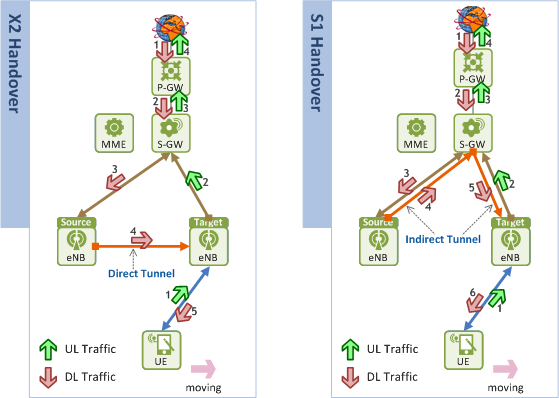
\includegraphics[width=.7\textwidth]{image/week11/3-1.png}
	\caption{\small X2 based Handover and S1 based Handover}
	\vspace{-10pt}
\end{figure}